\documentclass[12pt, a4paper]{article}

\usepackage{import}
\usepackage{standalone}

\usepackage[top=4cm, right=2cm, bottom=2.7cm, left=2cm]{geometry}

\usepackage{wrapfig}
\usepackage{tabulary}
\usepackage{float}
\usepackage{pifont}
\usepackage{background}
\usepackage{tikz}


\pagestyle{empty}
\setlength{\parindent}{0pt}

\begin{document}
	\begin{minipage}{\textwidth}
		\section{Vertakte Fietsen \hfill\small Bron: Bebras}
			\begin{wrapfigure}{r}{0.42\textwidth} 
				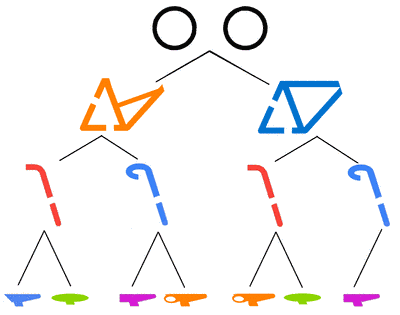
\includegraphics[width=\linewidth]{image1}
			\end{wrapfigure}
			Er is een nieuwe mode in Bevergem: je moet nu een veelvormige en veelkeurige fiets hebben. Maar om helemaal goed te zijn moet je de verschillende elementen van je fiets goed kiezen en vooral in de juiste combinatie.
			
			Het schema hiernaast beschrijft alle combinaties die nu in de mode zijn. Vertrek bij de twee wielen bovenaan en volg de lijnen naar beneden, naar links of naar rechts, om te weten welke onderdelen je mag kiezen en combineren.
			
			Welke van de fietsen hieronder \textbf{volgt niet} het schema dat we hiernaast hebben afgebeeld?
			\vspace{0.5cm}
			
			\begin{table}[H]
				\begin{tabulary}{\linewidth}{|C|C|C|C|}
					\hline
					\textbf{A} & \textbf{B} & \textbf{C} & \textbf{D} \\
					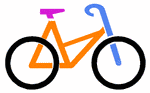
\includegraphics[width=\linewidth]{option1} &
					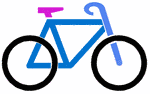
\includegraphics[width=\linewidth]{option2} &
					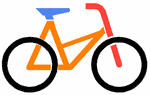
\includegraphics[width=\linewidth]{option3} &
					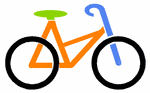
\includegraphics[width=\linewidth]{option4} \\
					\hline 
				\end{tabulary}
			\end{table}
	\end{minipage} \\ \\
		
\end{document}